\section{Mathematical Methods}

A small number of mathematical methods which may not be familiar to the reader are used within this thesis. They are outlined below.

\subsection{K-means clustering}

K-means clustering is a method for cluster analysis, whereby unsorted data is sorted into $k$ distinct groups based on proximity to evolving anchors. Figure \ref{fig:KM1lr} shows the results of a k-means clustering on unsorted data, with colours indicating output cluster designations. It can be seen that the chosen clusters align well with what may have been chosen by a human observer. In this case the groups are relatively well separated, and so the task to the k-means algorithm was relatively undemanding.

\begin{figure}[htbp]
 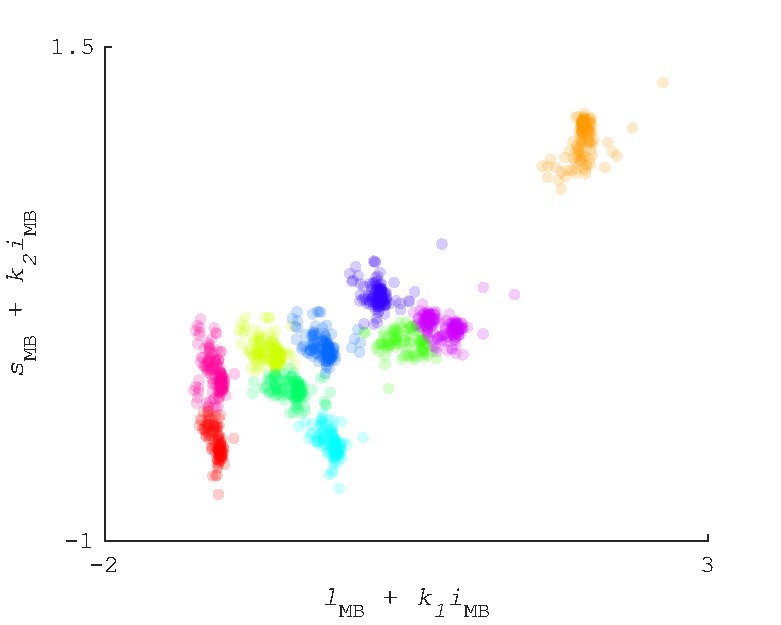
\includegraphics[max width=\textwidth]{figs/comp/KMeansMarkDemo/1.pdf}
 \caption{A reproduction of Figure \ref{fig:KM1} from Page \pageref{fig:KM1}, which shows the results of a k-means clustering of the data from Figure \ref{fig:corrected} from Page \pageref{fig:corrected} (which shows the \emph{actual} groups.}
 \label{fig:KM1lr}
\end{figure} 

The standard algorithm proceeds as follows: 

\begin{enumerate}
    \item $k$ random starting positions are assigned. 
    \item Each data-point is assigned a group based on which starting position is closest.
    \item The mean location of the data-points in each group is computed.
    \item Steps 2 and 3 are repeated, using the computed means instead of the original starting positions, until a stage where an iteration of these two steps results in no data-point changing groups. Once this occurs, the algorithm is said to have converged, and the resulting groupings are output.
\end{enumerate}

\subsection{Principal Component Analysis}

\textit{A valuable primer on \acrshort{PCA} in relation to colour technology is available from \citet{tzeng_review_2005}.}

\bigskip

\glsreset{PCA}
\Gls{PCA} is a dimensionality reduction method, used to to reduce the number of variables within a dataset whilst retaining as much of the variance as possible, and often used to identify the correlated roots of variance.

\begin{figure}[htbp]
 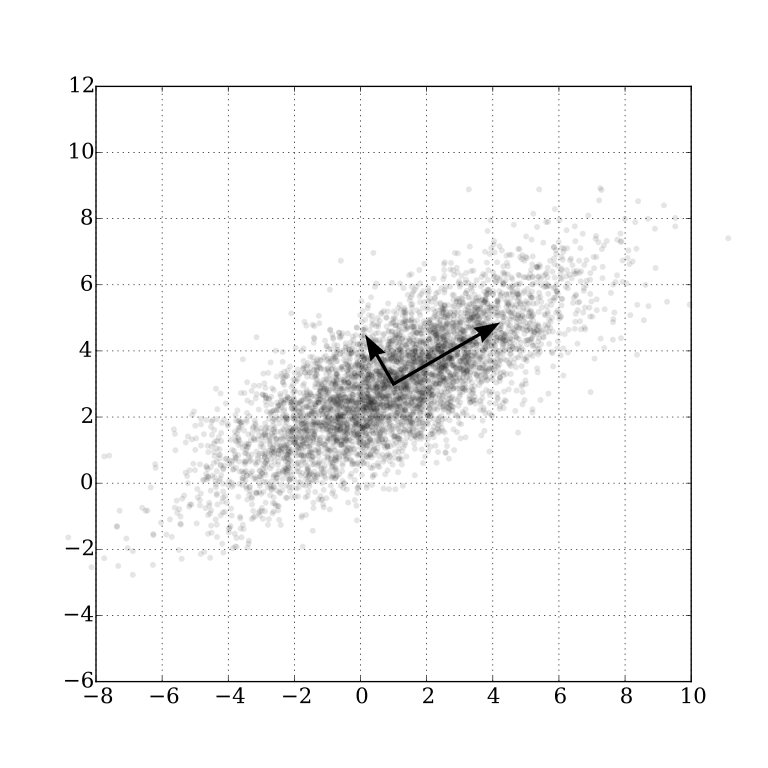
\includegraphics[max width=\textwidth]{figs/LitRev/PCA.png}
 \caption{Two-dimesional data with the first and second principal components added. Source: \url{https://commons.wikimedia.org/wiki/File:GaussianScatterPCA.svg}}
 \label{fig:PCA}
\end{figure} 

Along with similar techniques (such as single value decomposotion), it is used extensively within the study of daylight \glspl{SPD} \citep{hernandez-andres_color_2001,ojeda_influence_2012,pant_estimating_2009,bui_group_2004,judd_spectral_1964,maloney_computational_1984,spitschan_variation_2016} and natural \glspl{SRF} \citep{maloney_computational_1984,dzmura_color_1992,maloney_evaluation_1986,maloney_color_1986,cohen_dependency_1964,ferrero_principal_2011,zhang_reconstructing_2008,kwon_surface_2007,agahian_reconstruction_2008,harifi_recovery_2008,parkkinen_characteristic_1989,vrhel_color_1992,fairman_principal_2004,ayala_use_2006,eem_reconstruction_1994-2,connah_multispectral_2006,shi_using_2002,morovic_metamer-set-based_2006}. 

%A key goal for many of the researchers listed above... - how many dimensions/sensors do we need

In eras where the transmission of large datasets was troublesome, dimensionality reduction methods such as \gls{PCA} held value as a method to summarise a dataset, with the understanding that a reader could reconstruct a pseudo-dataset with minimal data-loss from the provided principal components. One such example is the work of \citet{judd_spectral_1964} where only the mean and first four characteristic vectors are provided\footnote{This is not technically \gls{PCA} but the related technique of \citet{morris_objective_1954}.}. The data from this study is replotted in Figure \ref{fig:Judd} and it can be seen that for their dataset this description does seem to offer a sensible summary of the data: the shape of the mean can be seen, and it can be seen that further variation principally occurs as a result of $V_{2}$ which is a broad and relatively monotonic function, indicating that changes are likely to be a skewing of the spectral shape.

\begin{figure}[htbp]
 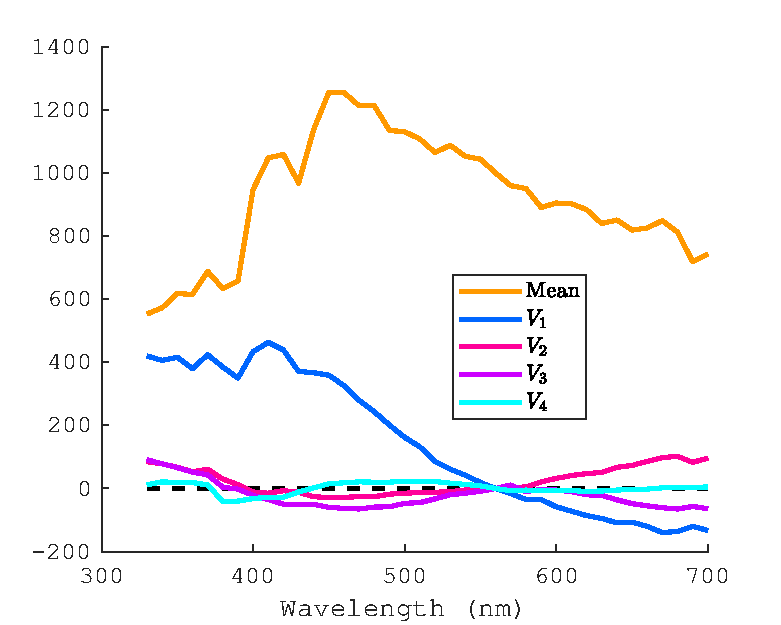
\includegraphics[max width=\textwidth]{figs/LitRev/Judd.pdf}
 \caption{The mean and first four characteristic vectors of \citet{judd_spectral_1964}.}
 \label{fig:Judd}
\end{figure} 